\documentclass[11pt,openany]{article}

\usepackage{mathtools, commath}
% Packages for formatting
\usepackage[margin=1in]{geometry}
\usepackage{fancyhdr}
\usepackage{enumerate}
\usepackage{graphicx}
\usepackage{kotex}
\usepackage{arydshln} % Include this package
\usepackage{bbding}
\usepackage{amsmath}
\usepackage{amsthm}
\usepackage[dvipsnames,table]{xcolor}
\usepackage{amssymb, amsfonts}
\usepackage{wasysym}
\usepackage{footnote}
\usepackage{tablefootnote}
\usepackage{arydshln} % Include this package
% Fonts
\usepackage[T1]{fontenc}
\usepackage[utf8]{inputenc}
\usepackage{newpxtext,newpxmath}
\usepackage{sectsty}

% Define colors
\definecolor{TealBlue1}{HTML}{0077c2}
\definecolor{TealBlue2}{HTML}{00a5e6}
\definecolor{TealBlue3}{HTML}{b3e0ff}
\definecolor{TealBlue4}{HTML}{00293c}
\definecolor{TealBlue5}{HTML}{e6f7ff}

\definecolor{thmcolor}{RGB}{231, 76, 60}
\definecolor{defcolor}{RGB}{52, 152, 219}
\definecolor{lemcolor}{RGB}{155, 89, 182}
\definecolor{corcolor}{RGB}{46, 204, 113}
\definecolor{procolor}{RGB}{241, 196, 15}

\usepackage{color,soul}
\usepackage{soul}
\newcommand{\mathcolorbox}[2]{\colorbox{#1}{$\displaystyle #2$}}
\usepackage{cancel}
\newcommand\crossout[3][black]{\renewcommand\CancelColor{\color{#1}}\cancelto{#2}{#3}}
\newcommand\ncrossout[2][black]{\renewcommand\CancelColor{\color{#1}}\cancel{#2}}

\usepackage{hyperref}
\usepackage{booktabs}

% Chapter formatting
\definecolor{titleTealBlue}{RGB}{0,53,128}
\usepackage{titlesec}
\titleformat{\section}
{\normalfont\sffamily\Large\bfseries\color{titleTealBlue!100!gray}}{\thesection}{1em}{}
\titleformat{\subsection}
{\normalfont\sffamily\large\bfseries\color{titleTealBlue!50!gray}}{\thesubsection}{1em}{}

%Tcolorbox
\usepackage[most]{tcolorbox}
\usepackage{multirow}
\usepackage{multicol}

\usepackage[linesnumbered,ruled]{algorithm2e}
\usepackage{algpseudocode}
\usepackage{setspace}
\SetKwComment{Comment}{/* }{ */}
\SetKwProg{Fn}{Function}{:}{end}
\SetKw{End}{end}
\SetKw{DownTo}{downto}

% Define a new environment for algorithms without line numbers
\newenvironment{algorithm2}[1][]{
	% Save the current state of the algorithm counter
	\newcounter{tempCounter}
	\setcounter{tempCounter}{\value{algocf}}
	% redefine the algorithm numbering (remove prefix)
	\renewcommand{\thealgocf}{}
	\begin{algorithm}
	}{
	\end{algorithm}
	% Restore the algorithm counter state
	\setcounter{algocf}{\value{tempCounter}}
}

\usepackage{adjustbox}
% Header and footer formatting
\pagestyle{fancy}
\fancyhead{}
\fancyhf{}
\rhead{\textcolor{TealBlue2}{\large\textbf{기대수(기초부터 대학원 수학까지 시리즈) 3기}}}%\rule{3cm}{0.4pt}}
\lhead{\textcolor{TealBlue2}{\large\textbf{수학의 즐거움, Enjoying Math}}}
% Define footer
%\newcommand{\footer}[1]{
%\begin{flushright}
%	\vspace{2em}
%	\includegraphics[width=2.5cm]{school_logo.jpg} \\
%	\vspace{1em}
%	\textcolor{TealBlue2}{\small\textbf{#1}}
%\end{flushright}
%}
%\rfoot{\large Department of Information Security, Cryptogrphy and Mathematics, Kookmin Uni.\includegraphics[height=1.5cm]{school_logo.jpg}}
\fancyfoot{}
\fancyfoot[C]{-\thepage-}

\usepackage{tcolorbox}
\tcbset{colback=white, arc=5pt}

\definecolor{axiomcolor}{HTML}{a88bfa}
\definecolor{defcolor}{RGB}{52, 152, 219}
\definecolor{procolor}{RGB}{241, 196, 15}
\definecolor{thmcolor}{RGB}{231, 76, 60}
\definecolor{lemcolor}{RGB}{155, 89, 182}
\definecolor{corcolor}{RGB}{46, 204, 113}
\definecolor{execolor}{RGB}{90, 128, 127}

% Define a new command for the custom tcolorbox
\newcommand{\axiombox}[2][]{%
	\begin{tcolorbox}[colframe=axiomcolor, title={\color{white}\bfseries #1}]
		#2
	\end{tcolorbox}
}

\newcommand{\defbox}[2][]{%
	\begin{tcolorbox}[colframe=defcolor, title={\color{white}\bfseries #1}]
		#2
	\end{tcolorbox}
}

\newcommand{\lembox}[2][]{%
	\begin{tcolorbox}[colframe=lemcolor, title={\color{white}\bfseries #1}]
		#2
	\end{tcolorbox}
}

\newcommand{\probox}[2][]{%
	\begin{tcolorbox}[colframe=procolor, title={\color{white}\bfseries #1}]
		#2
	\end{tcolorbox}
}

\newcommand{\thmbox}[2][]{%
	\begin{tcolorbox}[colframe=thmcolor, title={\color{white}\bfseries #1}]
		#2
	\end{tcolorbox}
}

\newcommand{\corbox}[2][]{%
	\begin{tcolorbox}[colframe=corcolor, title={\color{white}\bfseries #1}]
		#2
	\end{tcolorbox}
}



\usepackage{amsthm}

% Define custom theorem styles
\newtheoremstyle{dotless} % Name of the style
{3pt} % Space above
{3pt} % Space below
{\itshape} % Body font
{} % Indent amount
{\bfseries} % Theorem head font
{} % Punctuation after theorem head
{2.5mm} % Space after theorem head
{} % Theorem head spec

\newtheoremstyle{definitionstyle} % Name of the style
{3pt} % Space above
{3pt} % Space below
{} % Body font
{} % Indent amount
{\bfseries} % Theorem head font
{.} % Punctuation after theorem head
{2.5mm} % Space after theorem head
{} % Theorem head spec

% Applying custom styles
\theoremstyle{dotless}
\newtheorem{theorem}{Theorem} % Theorem environment with section-wise numbering
\newtheorem{proposition}[theorem]{Proposition} % Theorem environment with section-wise numbering
\newtheorem{lemma}[theorem]{Lemma} % Lemma shares the counter with theorem
\newtheorem{corollary}[theorem]{Corollary} % Corollary shares the counter with theorem

\theoremstyle{definitionstyle}
\newtheorem*{observation}{\textcolor{Magenta}{Observation}}
\newtheorem{definition}{Definition} % Definition shares the counter with theorem
\newtheorem{example}{Example} % Example shares the counter with theorem
\newtheorem{exercise}{Exercise} % Example shares the counter with theorem
\newtheorem{remark}{Remark} % Remark shares the counter with theorem
\newtheorem*{note}{Note}

\newtheorem*{definition*}{Definition} % Definition shares the counter with theorem
\newtheorem*{example*}{Example} % Example shares the counter with theorem
\newtheorem*{exercise*}{\textcolor{violet}{Exercise}} % Example shares the counter with theorem
\newtheorem*{remark*}{Remark} % Remark shares the counter with theorem


\usepackage{tikz}
\usepackage{tikz-cd}
\usepackage{tikz-3dplot}
\usepackage{pgfplots}
\pgfplotsset{compat=newest} % Adjust to your version of pgfplots
\def\Circlearrowleft{\ensuremath{%
		\rotatebox[origin=c]{180}{$\circlearrowleft$}}}
\def\Circlearrowright{\ensuremath{%
		\rotatebox[origin=c]{180}{$\circlearrowright$}}}
\def\CircleArrowleft{\ensuremath{%
		\reflectbox{\rotatebox[origin=c]{180}{$\circlearrowleft$}}}}
\def\CircleArrowright{\ensuremath{%
		\reflectbox{\rotatebox[origin=c]{180}{$\circlearrowright$}}}}
\usetikzlibrary{
	3d, % For 3D drawing
	angles,
	arrows,
	arrows.meta,
	backgrounds,
	bending,
	calc,
	decorations.pathmorphing,
	decorations.pathreplacing,
	decorations.markings,
	fit,
	matrix,
	patterns,
	patterns.meta,
	positioning,
	quotes,
	shadows,
	shapes,
	shapes.geometric,
	tikzmark
}
\tikzset{
	% single mid‐path arrow
	mid arrow/.style={
		decoration={
			markings,
			mark=at position 0.5 with {\arrow{Stealth[scale=1.2]}}
		},
		postaction={decorate},
	},
	% style for field arrows
	field arrow/.style={
		-{Stealth[scale=1.0]},
		thick,
		blue!70!black,
	},
}
\newcommand{\ie}{\textnormal{i.e.}}
\newcommand{\rsa}{\mathsf{RSA}}
\newcommand{\rsacrt}{\mathsf{RSA}\textendash\mathsf{CRT}}
\newcommand{\inv}[1]{#1^{-1}}

%New Command
%\newcommand{\set}[1]{\left\{#1\right\}}
\newcommand{\N}{\mathbb{N}}
\newcommand{\Z}{\mathbb{Z}}
\newcommand{\Q}{\mathbb{Q}}
\newcommand{\R}{\mathbb{R}}
\newcommand{\cR}{\mathcal{R}}
\newcommand{\C}{\mathbb{C}}
\newcommand{\F}{\mathbb{F}}
\newcommand{\nbhd}{\mathcal{N}}
\newcommand{\Log}{\operatorname{Log}}
\newcommand{\Arg}{\operatorname{Arg}}
\newcommand{\pv}{\operatorname{P.V.}}

\newcommand{\of}[1]{\left( #1 \right)} 
%\newcommand{\abs}[1]{\left\lvert #1 \right\rvert}
%\newcommand{\norm}[1]{\left\| #1 \right\|}

\newcommand{\sol}{\textcolor{magenta}{\bf Sol}}
\newcommand{\conjugate}[1]{\overline{#1}}

\newcommand{\res}{\operatorname{res}}
\DeclareMathOperator*{\Res}{\operatorname{Res}}

%\renewcommand{\Re}{\operatorname{Re}}
%\renewcommand{\Im}{\operatorname{Im}}

\newcommand{\cyclic}[1]{\langle #1 \rangle}
\newcommand{\uniform}{\overset{\$}{\leftarrow}}
\newcommand{\xmark}{\textcolor{red}{\XSolidBrush}}
\newcommand{\vmark}{\textcolor{green!75!black}{\CheckmarkBold}}

\newcommand{\gen}[1]{\langle #1 \rangle}
\newcommand{\Gen}[1]{\left\langle #1 \right\rangle}

\newcommand{\img}[1]{\text{Img}(#1)}
\newcommand{\Img}[1]{\text{Img}\left(#1\right)}
\newcommand{\preimg}[1]{\text{Img}^{-1}(#1)}
\newcommand{\Preimg}[1]{\text{Img}^{-1}\left(#1\right)}

\newcommand{\relation}{\mathrel{\mathcal{R}}}
\newcommand{\injection}{\rightarrowtail}
\newcommand{\surjection}{\twoheadrightarrow}
\newcommand{\id}{\textnormal{id}}

\newcommand{\eqclass}[1]{\left[#1\right]}

% Define custom colors for O and X
\newcommand{\yes}{\textcolor{blue}{\bf \fullmoon}}
\newcommand{\no}{\textcolor{red}{\bf \texttimes}}

\DeclarePairedDelimiter\ceil{\lceil}{\rceil}
\DeclarePairedDelimiter\floor{\lfloor}{\rfloor}
%\renewcommand{\floor}[#1]{\lfloor #1\rfloor}
%\newcommand{\Floor}[#1]{\left\lfloor #1\right\rfloor}
%\newcommand{\ceil}[#1]{\lceil #1\rceil}
%\newcommand{\Ceil}[#1]{\left\lceil #1\right\rceil}

\newcommand{\topology}{\mathscr{T}}
\newcommand{\sequence}[1]{\langle #1\rangle}
\renewcommand{\vec}[1]{\mathbf{#1}}
\setstretch{1.25}
\begin{document}
\pagenumbering{arabic}
\begin{center}
	\huge\textbf{Algebraic Structures}\\
	\vspace{0.5em}
	\large{Ji, Yong-hyeon}\\
%	\large{\ttfamily \url{https://github.com/Hacker-Code-J}}\\
	\vspace{0.5em}
	\normalsize{\today}\\
\end{center}

\noindent 
We cover the following topics in this note.
\begin{itemize}
	\item Group, Ring, Field
	\item Module, Vector Space, Algebra
\end{itemize}
\hrule\vspace{12pt}
%\tableofcontents
%\newpage

\begin{figure}[h!]\centering
%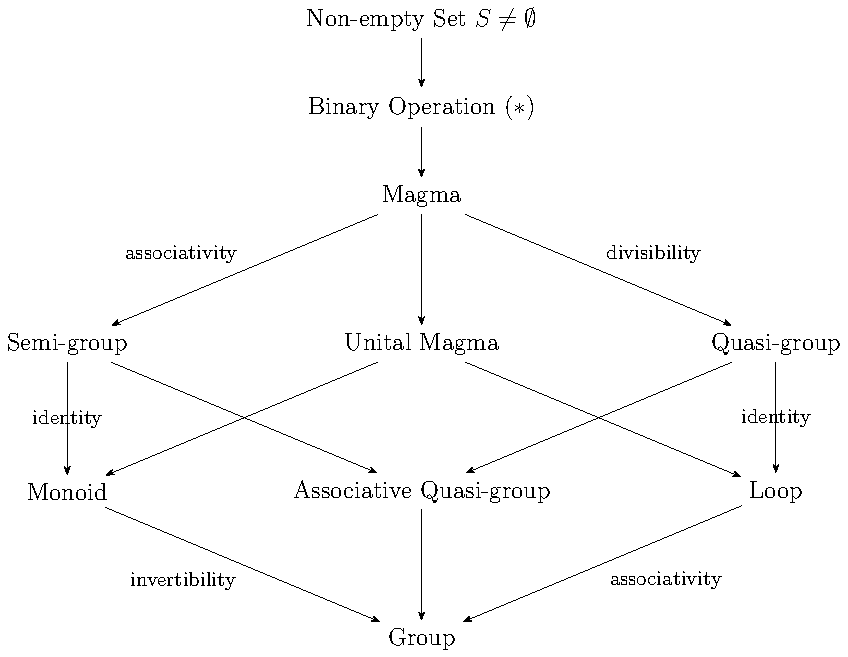
\includegraphics[width=\textwidth]{../tikz/grad-math-tikz-algebra/magamaTogroup.pdf}
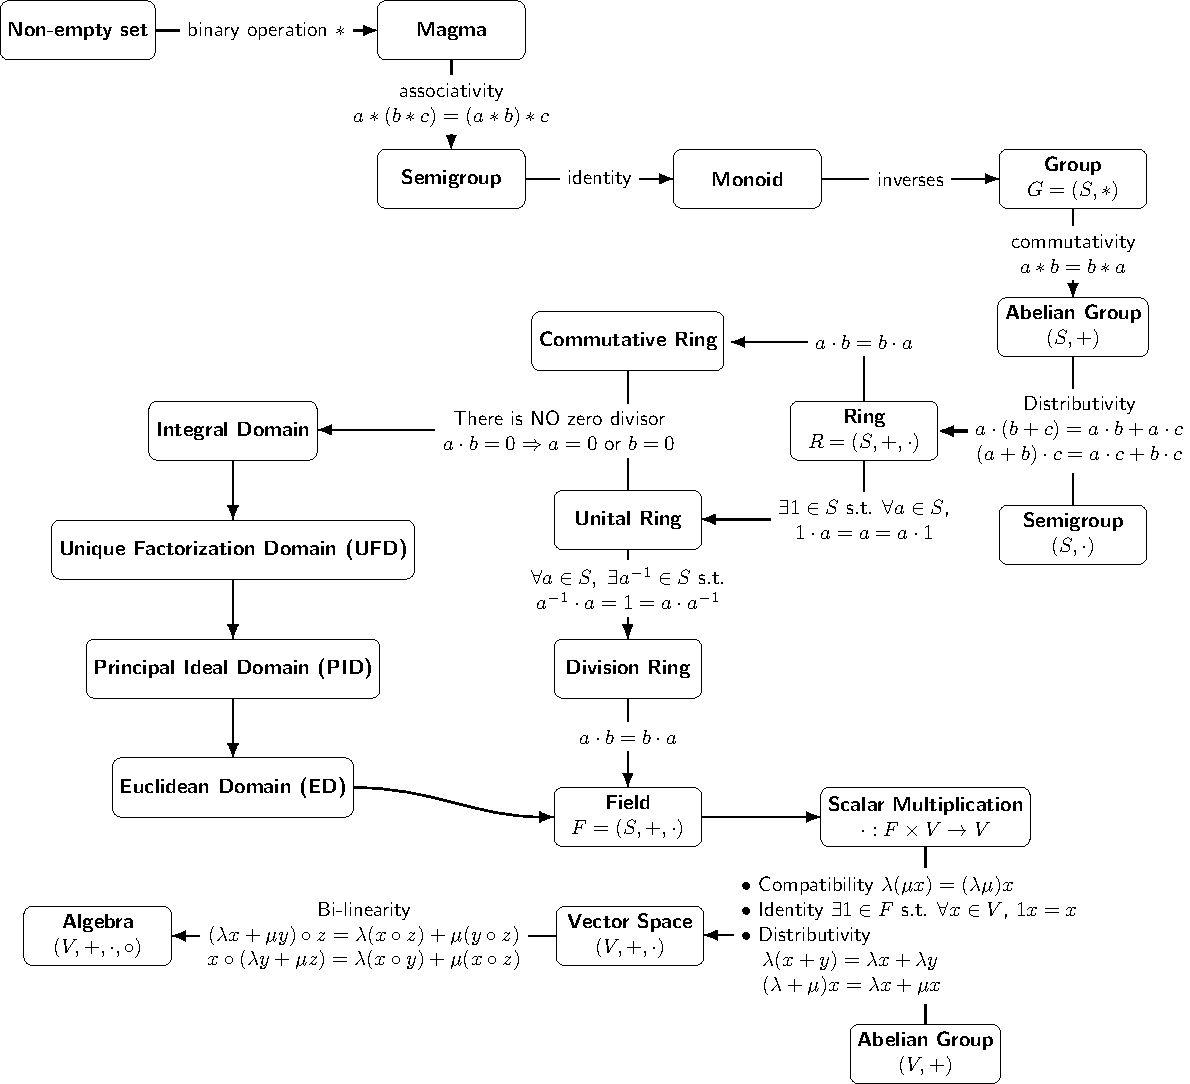
\includegraphics[width=\textwidth]{../tikz/grad-math-tikz-algebra/algebraic_structure.pdf}
\caption{Algebraic Structures}
\end{figure}
%\vspace{20pt}
%Algebraic structures are defined by sets equipped with one or more operations that satisfy specified axioms. These axioms guarantee, for example, that equations involving the operations behave in predictable ways. In this article we examine how the equation
%\[
%a\ast b = c
%\]
%(or its suitable variant) is interpreted in each context. We provide examples showing:
%\begin{itemize}
%	\item In a \emph{semigroup} the operation is associative and closed,
%	\item In a \emph{monoid} an identity element exists,
%	\item In a \emph{group} every element has an inverse (yielding unique solutions),
%	\item In a \emph{module} equations can involve both the additive structure and scalar multiplication over a ring,
%	\item In a \emph{vector space} (a module over a field) the additional invertibility of nonzero scalars facilitates solving linear equations.
%\end{itemize}
\newpage
\defbox[Binary Operation]{\begin{definition*}
Let \( S \) be a nonempty set. A \textbf{binary operation on} \( S \) is a function \[
* : S \times S \to S,
\] which assigns to each ordered pair $(a,b)\in S\times S$ an element $
*(a,b) = a*b\in S.$
\end{definition*}}
\begin{center}
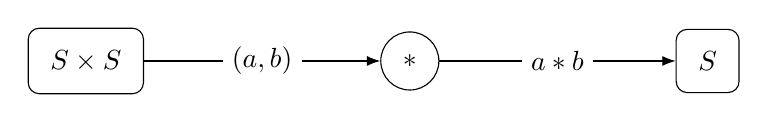
\begin{tikzpicture}[node distance=3cm, >=Latex]
	% Domain node
	\node (domain) [draw, rectangle, rounded corners, inner sep=8pt] {\(S \times S\)};
	% Operation node
	\node (op) [draw, circle, right=of domain, inner sep=5pt] {\( * \)};
	% Codomain node
	\node (codomain) [draw, rectangle, rounded corners, right=of op, inner sep=8pt] {\(S\)};
	
	% Arrows between nodes
	\draw[->] (domain) -- node[fill=white] {$(a,b)$} (op);
	\draw[->] (op) -- node[fill=white] {$a*b$} (codomain);
\end{tikzpicture}
\end{center}
\begin{example}
A binary operation on a set $S$ is a rule that assigns to every ordered pair 
$(a,b)\in S$ an element $a*b\in S$. \begin{itemize}
	\item (\emph{Addition on Integers}) Let $S=\Z$ and define \[
	+:\Z\times\Z\to\Z,\quad (a,b)\mapsto +(a,b)=a+b.
	\] This rule is a binary operation because the sum of any two integers is an integer.
	\vspace{20pt}
	\item (\emph{Maximum of Two Real Numbers}) Let $S=\R$ and define \[
	\fullfunction{\max}{\R\times\R}{\R}{(a,b)}{\max\set{a,b}}.
	\] For any two real numbers, their maximum is again a real number, so this is a valid binary operation.
\end{itemize}
\end{example}

\newpage
\defbox[Semi-group]{\begin{definition*}
A \textbf{semigroup} is an algebraic structure $(S,*)$ where:
\begin{enumerate}[(i)]
	\item $S\neq\varnothing$;
	\item $*:S\times S\to S$ is a binary operation that is \textit{associative}: for all $a,b,c\in S$, \[
	(a*b)*c\;=\; a*(b*c).
	\]
\end{enumerate}
\end{definition*}}

\begin{example}
A semigroup $(S,*)$ is a set $S$ together with a binary operation $*$ that is associative. \begin{itemize}
	\item (\emph{Positive Integers under Addition}) Let $S=\Z^+=\set{1,2,3,\dots}$ and define addition as the operation. For $a,b,c\in\Z^+$, \[
	(a+b)+c=a+(b+c).
	\] and the sum of two positive integers is again a positive integer.
	\vspace{20pt}
	\item (\textit{The Set $\set{0,1}$ under Multiplication}) We consider the set \[
	S=\set{0,1}\quad(\text{or}\ \Z_2\ \text{or}\ \F_2)
	\] and define binary operation $\times:S\times S\to S$ by the usual multiplication of numbers. That is, $\forall a,b\in S$, \[
	a\times b=\begin{cases}
		0 &:a=0\ \text{or}\ b=0\\
		1 &:a=1\ \text{and}\ b=1
	\end{cases}.
	\] The multiplication table for $S$ is \begin{table}[h!]\centering
		\begin{tabular}{c||c|c}
			$\times$ & 0 & 1 \\ \hline\hline
			0 & 0 & 0 \\ \hline
			1 & 0 & 1 \\
		\end{tabular}
	\end{table}\\ We check that $(S,\times)$ is a semigroup: \begin{itemize}
	\item Closure: For $a,b\in S$, the product $a\times b$ is either $0$ or $1$; hence $a\times b\in S$.
	\item Associativity: The operation is associative.
\end{itemize} Note that $(S,\times)$ is in fact a \textit{monoid} since there is the multiplicative identity $1$ s.t. \[
1\times a=a=a\times1\quad\text{for all $a\in S$}.
\]
	\vspace{20pt}
	\item (\emph{Singular Matrices under Matrix Multiplication}) Let \[
	S:=\set{A\in M_{n\times n}(\R):\det(A)=0},\ \text{the set of all $n\times n$ singular matrices over $\R$},
	\] the set of all $n\times n$ singular matrices over $\R$, and define the operation as matrix multiplication.
	\begin{itemize}
		\item Closure: If $A$ and $B$ are singular, then $\det(AB)=\det(A)\det(B)=0$; hence, $AB$ is singular.
		\item Associativity: Matrix multiplication is associative.
	\end{itemize}
	Since the identity matrix (which is non-singular) is not in $S$, this semigroup does not have an identity element.
\end{itemize}
\end{example}
\vspace{40pt}
\defbox[Monoid]{\begin{definition*}
A \textbf{monoid} is a semigroup \((S,\ast)\) that contains the \textit{identity element}. That is, there exists the element $e\in S$ such that for all $a\in S$. \[
e \ast a \;=\; a \;=\; a \ast e.
\]
\end{definition*}}
\begin{example}
A monoid is a semigroup that also has an identity element. \begin{itemize}
	\item (Nonnegative Integers under Addition) Let $S=\Z_{\geq 0}=\set{0,1,2,\dots}$ and define addition on $\Z_{\geq 0}$. \begin{itemize}
		\item Associativity: Addition is associative.
		\item Identity: The element $0\in\Z_{\geq 0}$ is the identity since \[
		0+a=a+0=a\quad \text{for each}\ a\in\Z_{\geq 0}.
		\]
	\end{itemize}
	\vspace{20pt}
	\item (All Square Matrices under Multiplication) Let $S=M_n(\R)$, the set of all $n\times n$ matrices with real entries, and define the operation as matrix multiplication. \begin{itemize}
		\item Associativity: Matrix multiplication is associative.
		\item Identity: The identity matrix $I_n$ (with ones on the diagonal and zeros elsewhere) satisfies \[
		I_nA=A=AI_n\quad\text{for all}\ A\in M_n(\R).
		\]
	\end{itemize}
\end{itemize}
\end{example}


\defbox[Group]{\begin{definition*}
A \textbf{group} is a monoid \((S,\ast)\) in which every element has the \textit{inverse}. That is, for all $a\in S$, there exists the element $b\in S$ such that
\[
a \ast b \;=\; e \;=\; b\ast a.
\] Such \( b \in S \) is called an \emph{inverse} of \( a \), and is commonly denoted \( b=a^{-1} \).
\end{definition*}}
\begin{remark}
A \textbf{group} is an algebraic structure $(G,*)$ satisfying the following axioms:
\begin{enumerate}[(G1)]
	\item[\textcolor{gray}{(G0)}] \textcolor{gray}{(Closure) $\forall a,b\in G,\ a*b\in G$;}
	\item (Associativitiy) $\forall a,b,c\in G,\ (a*b)*c=a*(b*c)$;
	\item (Identity) $\exists e\in G:\forall a\in G,\ a*e=a=e*a$;
	\item (Inverse) $\forall a\in G,\ \exists\inv{a}\in G:\inv{a}*a=e=a*\inv{a}$.
\end{enumerate}
\end{remark}
\vspace{40pt}
\begin{example}
A group $(G,*)$ is a monoid in which every element has the inverse. \begin{itemize}
	\item (Integers under Addition) Let $G=\Z$ and define addition on $\Z$. \begin{itemize}
		\item Associativity: Addition is associative;
		\item Identity: The integer $0$ is the identity;
		\item Inverse: For every $a\in\Z$, the element $-a\in\Z$ is its inverse since $a+(-a)=0=(-a)+a$. 
	\end{itemize}
	This group is abelian because addition is commutative.
	\vspace{20pt}
	\item (Bijections under Composition) Let $X$ be a nonempty set. Consider the set \[
	G=\mathcal{F}:=\set{f\in X^X:f\ \text{is a bijection}}.
	\] Define the binary operation $\circ$ as the composition of functions. The structure $(\mathcal{F},\circ)$ forms a group: \begin{itemize}
		\item Associativity: Composition is associative.
		\item Identity: $\text{id}_X:X\to X$, $x\mapsto x$ for all $x\in X$.
		\item Inverse: Every bijection $f$ has an inverse function $f^{-1}$.
 	\end{itemize}
	\item (General Linear Group) Let \[
	G=GL(n,\R)=\set{A\in M_n(\R):\det(A)\neq 0},
	\] with the operation of matrix multiplication. \begin{itemize}
		\item Associativity: Matrix multiplication is associative.
		\item Identity: The identity matrix $I_n$ is the identity.
		\item Inverse: Every matrix in $GL(n,\R)$ is invertible. This group is generally non-abelian.
	\end{itemize}
\end{itemize}
\end{example}
\vspace{40pt}
\begin{remark}
A group $(G,*)$ is called an \textbf{abelian group} (or \textbf{commutative group}) if the binary operation $*$ is \textit{commutative}; that is, for all $a,b\in G$,
\[
a * b = b * a,
\]
\end{remark}
\vspace{20pt}
\begin{example}[Lie-bracket]
Let $\mathfrak{g}$ be a vector space over a field $F$. A \textbf{Lie bracket} on $\mathfrak{g}$ is a bilinear map \[
\fullfunction{[\cdot,\cdot]}{\mathfrak{g}\times\mathfrak{g}}{\mathfrak{g}}{(x,y)}{[x,y]=xy-yx}.
\] Then, for all $x,y,z\in\mathfrak{g}$, \begin{align*}
[x,[y,z]]&=[x,yz-zy]=x(yz-zy)-(yz-zy)x=xyz-xzy-yzx+zyx,\\
[[x,y],z]&=[xy-yx,z]=(xy-yx)z-z(xy-yx)=xyz-yxz-zxy+zyx.
\end{align*} Thus, Lie bracket is \textit{not} associative.
\end{example}

\newpage
\probox[Left and Right Cancellation]{\begin{proposition}
Let $G$ be a group, and let $a,b,c,d\in G$. Let $e\in G$ is the identity of $G$. \begin{enumerate}[(1)]
	\item (Left Cancellation) $ca=cb\implies a=b$.
	\item (Right Cancellation) $ac=bc\implies a=b$.
	\item $ab=e\iff ba=e$
\end{enumerate}
\end{proposition}}
\begin{proof}
\begin{enumerate}[(1)]
	\item $ca=cb\implies c^{-1}(ca)=c^{-1}(cb)\implies(c^{-1}c)a=(c^{-1}c)b\implies ea=eb\implies a=b$.
	\item $ac=bc\implies (ac)c^{-1}=(bc)c^{-1}\implies a(cc^{-1})=b(cc^{-1})\implies ae=be\implies a=b$.
	\item \begin{itemize}
		\item[($\Rightarrow$)] $ab=e\implies a^{-1}(ab)=a^{-1}e\implies b=a^{-1}\implies ba=e$
		\item[($\Leftarrow$)] $ba=e\implies b^{-1}(ba)=b^{-1}e\implies a=b^{-1}\implies ab=e$
	\end{itemize}
\end{enumerate}
\end{proof}
\vspace{40pt}
\probox[Uniqueness of Identity and Inverse]{\begin{proposition}
Let $G$ be a group. \begin{enumerate}[(1)]
	\item The identity $e\in G$ is unique.
	\item For each $a\in G$, the inverse $a^{-1}\in G$ is unique.
\end{enumerate}
\end{proposition}}
\begin{proof}
\begin{enumerate}[(1)]
	\item Let $e,e'$ are identities of $G$. Then \[
	e\;\tikzmarknode{m1}{=}\;ee'\;\tikzmarknode{m2}{=}\;e'.
	\]
	\begin{tikzpicture}[remember picture, overlay, font=\sffamily]
		\node[draw=green!70!black, thick, fit=(m1), inner xsep=1pt](box1){};
		\draw[thick, green!70!black] (box1)--++(0,-.6)--++(-1,0) node[left, scale=.75]{$e'$ is an identity of $G$};
		\node[draw=orange, thick, fit=(m2), inner xsep=1pt](box2){};
		\draw[thick, orange] (box2)--++(0,-.6)--++(1,0) node[right, scale=.75]{$e$ is an identity of $G$};
	\end{tikzpicture}
	\item Let $a_1^{-1},a_2^{-1}$ are inverses of $a\in G$. Then \[
	aa_1^{-1}=aa_2^{-1}\implies a_1^{-1}=a_2^{-1}\quad\text{by left cancellation law.}
	\] 
\end{enumerate}
\end{proof}

\defbox[Ring]{\begin{definition*}
A \textbf{ring} is an algebraic structure $(R,+,\cdot)$ where: \begin{enumerate}[(i)]
	\item $(R,+)$ is an abelian group with identity element $0$: that is, for all $a,b,c\in R$: \begin{itemize}
		\item Associativity: $(a+b)+c=a+(b+c)$;
		\item Commutativity: $a+b=b+a$;
		\item Identity: There exists $0\in R$ such that $a+0=a$;
		\item Inverse: For every $a\in R$, there exits an element $-a\in R$ with $a+(-a)=0$.
	\end{itemize}
	\item $(R,\cdot)$ is a semigroup; that is, multiplication is \textit{associative}: \[
	(a\cdot b)\cdot c=a\cdot (b\cdot c)\quad\text{for all}\ a,b,c\in R.
	\]
	\item Distributivity (Compatibility):\\
	 Multiplication is distributive over addition; that is, for all $a,b,c\in R$,\begin{align*}
		a\cdot (b+c)=a\cdot b+a\cdot c\quad\text{and} \quad
		(a+b)\cdot c=a\cdot c+b\cdot c.
	\end{align*} 
\end{enumerate}
\end{definition*}\tcblower
\color{gray!50} Some authors require the existence of a multiplicative identity (an element $1\in R$ such that $1\cdot a=a=a\cdot 1$ for all $a\in R$); if so, the ring is called a ring with unity.}
\begin{example}
\ \begin{itemize}
	\item (The Integers $\Z$) Consider $R=\Z$ with the usual addition and multiplication.
	\begin{itemize}
		\item $(\Z,+)$ is an abelian group (with identity $0$).
		\item Multiplication is associative.
		\item The distributive laws hold, \ie, $a(b+c)=ab+ac$ and $(a+b)c=ac+bc$ for all $a,b,c\in\Z$.
	\end{itemize}
	This ring is also commutative and has a multiplicative identity $1$.
	\vspace{20pt}
	\item (Polynomial Ring $\C[x]$) Let $R=\C[x]$, the set of all polynomials in $x$ with complex coefficients. \begin{itemize}
		\item $(\C[x],+)$ is an abelian group (with the zero polynomial $0$ as the identity).
		\item Polynomial multiplication is associative.
		\item The distributive laws hold, \ie, $f(x)(g(x)+h(x))=f(x)g(x)+f(x)h(x)$ and $(f(x)+g(x))h(x)=f(x)h(x)+g(x)h(x)$ for all $f(x),g(x),h(x)\in\C[x]$.
	\end{itemize}
	This ring is also commutative and has a multiplicative identity $1$ (the constant polynomial $1$).
\end{itemize}
\end{example}

\defbox[Field]{\begin{definition*}
A \textbf{field} an algebraic structure $(F,+,\cdot)$ such that \begin{enumerate}[(i)]
	\item $(F,+)$ is an abelian group with additive identity element $0$;
	\item $(F\setminus\set{0},\cdot)$ is a commutative group with multiplicative identity element $1$, where $0\neq 1$;
	\item Distributivity: Multiplication is distributive over addition; that is, for all $a,b,c\in F$, \[
	a\cdot (b+c)=a\cdot b+a\cdot c.
	\]
\end{enumerate} 
\end{definition*}\tcblower A field $F$ is a commutative division ring.}
\begin{remark}
 A field is the smallest algebraic structure in which we can perform all the arithmetic operations $+,-,\times,\div$ (division by nonzero element), so in particular every nonzero element must a the multiplicative inverse.
\end{remark}
\vspace{40pt}
\begin{example}
A field is a commutative ring with unity in which every nonzero element is invertible under multiplication. \begin{itemize}
	\item (The Real Numbers $\R$) Let $F=\R$ with the usual addition and multiplication. \begin{itemize}
		\item $(\R,+)$ is an abelian group (with $0$ as the additive identity)
		\item $(\R\setminus\set{0},\cdot)$ is an commutative group (with $1$ as the multiplicative identity)
		\item Multiplicative distributes over addition.
	\end{itemize}
	\vspace{20pt}
	\item (Finite Field $\Z_p$) Let $p$ be a prime number and define \[
	\Z_p:=\set{0,1,\dots, p-1},
	\] with addition and multiplication defined modulo $p$. \begin{itemize}
		\item $(\Z_p,+)$ is an abelian group with the additive identity $0$.
		\item $(\Z_p\setminus\set{0},\cdot)$ is a commutative group with the multiplicative identity $1$ since every nonzero element has a unique inverse module $p$\footnote{By Bézout's identity, for $a,b\in\Z$, $\exists x,y\in\Z$ s.t. $ax+by=\gcd(a,b)$. Let $p$ be a prime. Then for any integer $a\in\Z$, $\exists x,y$ s.t. $ax+py=\gcd(a,p)=1$, and so $ax\equiv 1\pmod{p}$.}.
		\item The distributive laws hold.
	\end{itemize}
\end{itemize}
\end{example}
\vfill 
\newpage
\defbox[Module]{\begin{definition*}
Let \( R \) be a ring with unity $1_R$. An $R$-\textbf{module} is an structure $(M,+,\cdot)$ consisting of an abelian group $(M,+)$ together with a scalar multiplication $
\cdot:R\times M\to M
$ that satisfies the following axioms for all $r,r_1,r_2\in R$ and $m,m_1,m_2\in M$:
\begin{enumerate}[(i)]
	\item[(i)\footnote{Distributivity over Module Addition}] $
	r \cdot (m_1+m_2) = r \cdot m_1 + r \cdot m_2$
	\item[(ii)\footnote{Distributivity over Ring Addition}] $
	(r_1+r_2) \cdot m = r_1 \cdot m + r_2 \cdot m$
	\item[(iii)\footnote{Associativity of Scalar Multiplication}] $
	(r_1r_2) \cdot m = r_1 \cdot (r_2 \cdot m)$
	\item[(iv)\footnote{Unital Property (if $R$ is unital)}] $
	1_R \cdot m = m.$
\end{enumerate}
\end{definition*}}
\begin{remark}
Consider $R$-module $(M,+,\cdot)$. Let $m\in M$. Since $0_R=0_R+0_R$, we have \[
0_R\cdot m=(0_R+0_R)\cdot m=0_R\cdot m+ 0_R\cdot m.
\] Then  \[
0_R\cdot m\textcolor{red}{\;-\; 0_R\cdot m}=0_R\cdot m+ 0_R\cdot m\textcolor{red}{\;-\; 0_R\cdot m},
\] and so $0_M=0_R\cdot m+0_M$, \ie, $0_M=0_R\cdot m$.
\end{remark}
\vfill
\defbox[Vector Space]{\begin{definition*}
Let \( F \) be a field. A \emph{vector space} over \( F \) is a structure \((V, +, \cdot)\) satisfying:
\begin{enumerate}[(i)]
	\item \((V, +)\) is an abelian group with identity element \( 0 \in V \).
	\item \(\cdot : F \times V \to V\) is a function called \emph{scalar multiplication}.
	\item The following axioms hold: for all $a,b\in F$ and $u,v\in V$,
	\begin{enumerate}[(a)]
		\item $a \cdot (u+v) = a \cdot u + a \cdot v$.
		\item $(a+b) \cdot v = a \cdot v + b \cdot v$.
		\item $a \cdot (b \cdot v) = (a b) \cdot v$.
		\item $1_F \cdot v = v$ where \(1_F\) denotes the multiplicative identity in \( F \).
	\end{enumerate}
\end{enumerate} In other words, we say $V$ is a vector space over a field $F$ if $V$ is a $F$-module
\end{definition*}}
\newpage
\defbox[Algebra over a Field]{\begin{definition*}
Let $F$ be a field. An \textbf{$F$-algebra} is a quadruple $(V,+,\cdot,\circ)$ where \begin{enumerate}[(i)]
	\item[(i)\footnote{Abelian Group Structure}] $(V,+)$ is an abelian group (with additive identity $0$).
	\item[(ii)\footnote{Vector Space Structure}] $(V,+,\cdot)$ is an $F$-vector space. That is, for all $x,y\in V$ and $\lambda,\mu\in F$, \begin{itemize}
		\item $\lambda\cdot (x+y)=\lambda\cdot x+\lambda\cdot y$,
		\item $(\lambda+\mu)x=\lambda\cdot x+\lambda\cdot x$,
		\item $(\lambda\mu)\cdot x=\lambda\cdot(\mu\cdot x)$,
		\item $1_F\cdot x=x$.
	\end{itemize}
	\item[(iii)\footnote{Algebra Multiplication}] There is a binary operation \[
	\circ:V\times V\to V,
	\] which is $F$-bilinear. That is, for all $x,y,z\in V$ and all $\lambda\in F$, \begin{align*}
		(\lambda x+y)\circ z=\lambda(x\circ z)+(y\circ z),\\
		x\circ (\lambda y+z)=\lambda(x\circ y)+(x\circ z).
	\end{align*}
%	Equivalently, the scalar multiplication and the algebra multiplication are compatible: \[
%	\lambda\cdot(x\circ y)=(\lambda\cdot x)\circ y=x\circ (\lambda\cdot y).
%	\]
\end{enumerate}
\end{definition*}\tcblower
An algebra $(V,\circ)$ over a ring $F$, where $F$ is a field and the $F$-module is a vector space. 
}

\vfill
\begin{thebibliography}{9}
	\bibitem{algebra_0}
	수학의 즐거움, Enjoying Math. ``수학 공부, 기초부터 대학원 수학까지, 13. 대수학 : 군, 환, 체, 가군, 벡터공간, 대수의 정의'' YouTube Video, 27:06. Published 
	October 7, 2019. URL: \url{https://www.youtube.com/watch?v=6DP6UQ2sPus}.
\end{thebibliography}

\end{document}
